\chapter{Example \LaTeX}

This chapter includes some example \LaTeX. 

Ever advancing developments in computational power... mean ever more pictures
of kittens on the internet. As you will see in Figure~\ref{fig:kittenpicture},
some of them are very cute.

\begin{figure}[H]
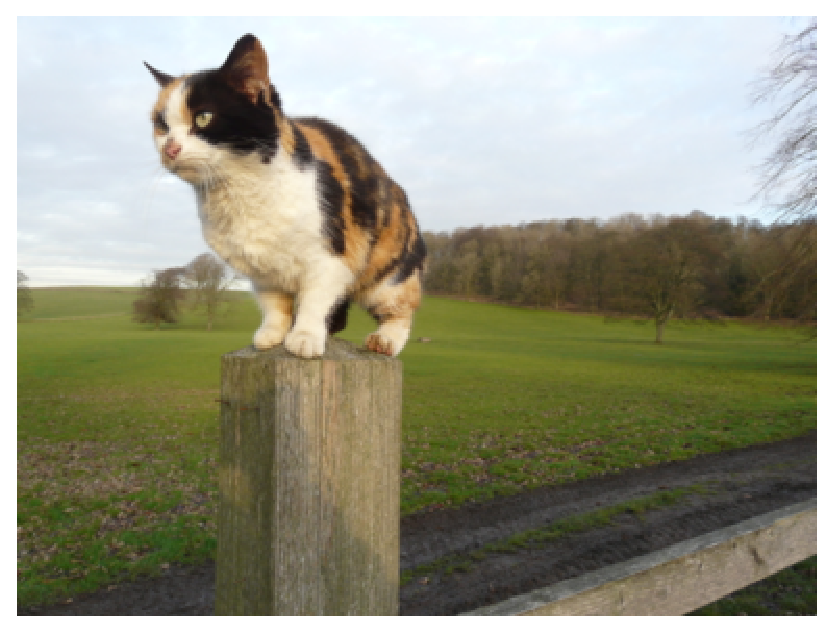
\includegraphics{Chapter7/kitten}
\caption{A picture of a kitten\cite{kittenpic_ref}.}
\label{fig:kittenpicture}
\end{figure}

\section{Overview}

In this section I am going to include a spurious label\label{spurious}, which
appears in the code but has no effect on the display at the time it was
inserted.  I am also going to include a spurious citation to a journal
article \cite{HannahsPaper}, a citation to a conference paper \cite{MarksPaper},
a citation to a book \cite{NumericalRecipes}, and a citation to a
website \cite{FailBlog}. All of these citations have been added to the BibTeX
(.bib) file which you'll find in the References directory -- they include some
tricky stuff (accents and so on) which are explained in the comments in the
BibTeX.


\subsection{A bit of extra text to give the section some bulk}

This is a paragraph of extra text just to make this section go over into a
second page and to show the use of headers and page numbering that happens
automatically once the text flows over to another page.  

\section{A few words of advice on \LaTeX}

One thing you should be aware of using \LaTeX\ is that \LaTeX\ has its own
ideas about where things should be placed and about where page breaks should
happen.  This minimises the chances of widow and orphan
text\footnote{\emph{Orphan} and \emph{Widow} text are when the last line of a
paragraph appears on the following page, or where a header appears on one page
and the following text appears on the next}, but it can lead to you feeling
like you've lost control if you're used to using software like Word.  The best
advice for text formatting is to just relax and relinquish control to \LaTeX;
for figures, it's a good idea to use the float package (already included in
this template) and put [H] after your includegraphics command.  You can see an
example of this usage in the code used to insert Figure~\ref{fig:kittenpicture}
on Page~\pageref{fig:kittenpicture}.

In the following paragraph, I've put a pointless equation. This is just so that you can see how to include an equation in a document. Equations are numbered separately, just like tables and figures.

\begin{equation}
X=\sum_{i=1}^{N} x_{i}+y_{i}
\label{eq:spurious}
\end{equation}

Like tables and figures, if you label an equation you can refer back to it
using the ref command (for the number of the equation) or the pageref command
(for the page the equation lies on).  The source for this document has examples
of both types of reference here: Equation~\ref{eq:spurious} lies on
Page~\pageref{eq:spurious}.

\section{Early work}

\begin{table}[H]
\begin{tabular}{l c l}
Year & Kitten frequency & Notes \\
\hline
1993 & 0.04& World wide web begins to become popular \\
1995 & 0.2 & Kittens take over\\
2008 & 0.34 & Cats make a stand\\
\end{tabular}
\caption{A pointless table, inserted to show that the list of tables will auto-update}
\end{table}

\subsection{The first signs of this topic}

In this section we have a spurious link back to a spurious label, which appeared in Section~\ref{spurious}.

% the use of ~ is a space that will not break over a line - use it
% after Section and Chapter to make sure it looks tidy




